\documentclass[../main.tex]{subfiles}
\begin{document}
    \chapter{Implementation of PHP type inference}\label{ch:inference_implementation}

    The type inference is executed in 3 main steps.
    The first step creates an $M^3$ model for a PHP program which contains various facts about the program. 
    The creation of an $M^3$ for PHP is explained in more details in section \ref{sec:m3_for_php}.
    Once the $M^3$ model is constructed, we extract constraints from the program using the $M^3$ model.
    Next, as explained in section \ref{sec:implementation:constraint_solving}, we solve the constraints and resolve the types of variables used in the program.
    The final section \ref{sec:implementation_additional_contraints} of this chapter explains how annotations and PHP built-in information is included in the process to improve the type inference.
    
    \section{$M^3$ for PHP}\label{sec:m3_for_php}
    As explained in section \ref{sec:background_rascal}, $M^3$ is a language independent meta model which holds facts about programs.
    The model can be extended with language specific elements and will be used to query the system for facts about the system.
    An overview how an $M^3$ for PHP is build is shown in figure \ref{fig:research_m3_creation}.
    Independent $M^3$ models are build each PHP file in the program.
    
    \begin{figure}[H]
        \centerline{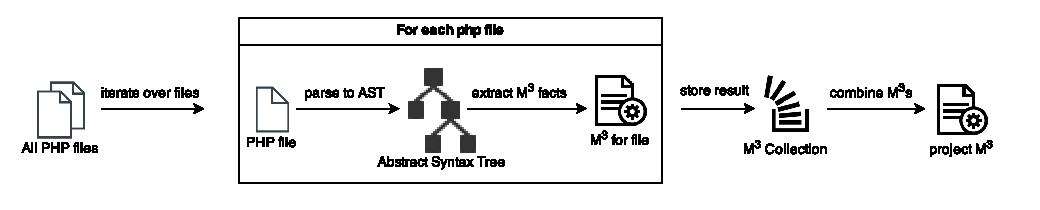
\includegraphics{Diagrams/M3Creation.pdf}}
        \caption{$M^3$ Creation}
        \label{fig:research_m3_creation}
    \end{figure}
    
    All these individual $M^3$'s are in the end combined to collect all the facts about a program.
    This results in one $M^3$ for the whole program.
    $M^3$'s are first created for each file is because it is not defined what the dependencies of a individual file are.
    There is no main file, and all files can load each other.
    In this research we assume that all files in a program are loaded when needed using autoloaders or manual includes.
    
    \subsection{Core elements}
    The $M^3$ model has the following core elements: \texttt{declarations}, \texttt{containment}, \texttt{modifiers}, \texttt{uses}, \texttt{names}, and \texttt{documentation}.
    The rascal code is displayed in Rascal \ref{fig:m3_core_elements}. The characteristics of the elements are described in the paragraphs below.

    \begin{program}    
    \begin{rascal}%%%%%%%%%%%%%%%%%%{ RASCAL }%%%%%%%%%%%%%%%%%%
\CAT{Keyword}{anno} \CAT{Keyword}{rel}{}[\CAT{Keyword}{loc} name, \CAT{Keyword}{loc} src] M3@declarations; \CAT{Comment}{// maps declarations to file location.}
\CAT{Keyword}{anno} \CAT{Keyword}{rel}{}[\CAT{Keyword}{loc} from, \CAT{Keyword}{loc} to] M3@containment; \CAT{Comment}{// what is logically contained in what else}
\CAT{Keyword}{anno} \CAT{Keyword}{rel}{}[\CAT{Keyword}{loc} definition, Modifier modifier] M3@modifiers; \CAT{Comment}{// associated modifiers}
\CAT{Keyword}{anno} \CAT{Keyword}{rel}{}[\CAT{Keyword}{loc} src, \CAT{Keyword}{loc} name] M3@uses; \CAT{Comment}{// maps src locations of usages to the declarations}
\CAT{Keyword}{anno} \CAT{Keyword}{rel}{}[\CAT{Keyword}{str} simpleName, \CAT{Keyword}{loc} qualifiedName] M3@names; \CAT{Comment}{// end-user readable names}
\CAT{Keyword}{anno} \CAT{Keyword}{rel}{}[\CAT{Keyword}{loc} definition, \CAT{Keyword}{loc} comments] M3@documentation; \CAT{Comment}{// comments and doc-blocks}\end{rascal}%%%%%%%%%%%%%%%%%%{ RASCAL }%%%%%%%%%%%%%%%%%%
	
	\caption{$M^3$ core definitions in Rascal}
	\label{fig:m3_core_elements}
	\end{program}
	    
    \paragraph{Declarations} \texttt{Declarations} defines the declarations of namespaces, classes, interfaces, methods, functions, and variables and holds the relation between the logical name (which is used to refer to the declaration) and the actual file location (which is the physical place in the file system.
    For example the logical name of a class can be \texttt{$\vert$php+class://SomeNameSpace/ClassX$\vert$} while the actual location might be \texttt{$\vert$file:///project/SomeNameSpace/ClassX.php$\vert$}.
    
    \paragraph{Containment} \texttt{Containment} holds information about what elements logically contain other elements.
    For example, a property or method is contained in a class and a class is contained in a package.
    When a function is declared in another function, they are both logically contained in the global namespace (the highest level) because all functions are declared as first class citizens in PHP.
    
    \paragraph{Modifiers} \texttt{Modifiers} element contains information about the modifiers of classes, fields, and methods. 
    Classes can only be \texttt{abstract}, fields can be \texttt{public}, \texttt{private}, or \texttt{protected}, and methods can be all of them. 
    Abstract methods can only be declared in abstract classes. 
    Classes are implicitly public.
    
    \paragraph{Uses} \texttt{Uses} relation holds information about the usages of certain elements.
    It is the relation between the usage and the declaration.
    For example when you instantiate a class, in that case you 'use' that specific class.
     
    \paragraph{Names} \texttt{Names} contains the declaration and a simplified version of the name.
    The declared name can be long and unreadable.
    \texttt{names} contains human readable name which can be used for presenting the element in a GUI.
    
    \paragraph{Documentation} \texttt{Documentation} contains the link to the documentation related to the source code element.
    The link is mapped to a declaration.
    
    \subsection{PHP specific elements}
    Because every programming language differs in syntax and semantics, the $M^3$ model is extensible to provide language specific elements.
    The following php specific items are added: \texttt{extends}, \texttt{implements}, \texttt{parameters}, \texttt{constructors}, and \texttt{annotations}.
    These PHP specific elements are described in more detail in the paragraphs below.

    \begin{program}    
    \begin{rascal}%%%%%%%%%%%%%%%%%%{ RASCAL }%%%%%%%%%%%%%%%%%%
\CAT{Keyword}{anno} \CAT{Keyword}{rel}{}[\CAT{Keyword}{loc} from, \CAT{Keyword}{loc} to] M3@extends;    \CAT{Comment}{// which class extends which class}
\CAT{Keyword}{anno} \CAT{Keyword}{rel}{}[\CAT{Keyword}{loc} from, \CAT{Keyword}{loc} to] M3@implements; \CAT{Comment}{// interface usages}
\CAT{Keyword}{anno} \CAT{Keyword}{rel}{}[\CAT{Keyword}{loc} decl, PhpParams params] M3@parameters; \CAT{Comment}{// formal functions/methods parameters}
\CAT{Keyword}{anno} \CAT{Keyword}{rel}{}[\CAT{Keyword}{loc} decl, \CAT{Keyword}{loc} to] M3@constructors; \CAT{Comment}{// constructor usages}
\CAT{Keyword}{anno} \CAT{Keyword}{rel}{}[\CAT{Keyword}{loc} pos, Annotation annotation] M3@annotations; \CAT{Comment}{// annotations from doc blocks}\end{rascal}%%%%%%%%%%%%%%%%%%{ RASCAL }%%%%%%%%%%%%%%%%%%
	
	\caption{PHP specific $M^3$ element}
	\label{fig:m3_php_elements}
	\end{program}
	    
	\paragraph{Extends} \texttt{Extends} contains information about what classes and interface extend other classes or interfaces.
	Please note that we do not hold information about which class implements which interface, because that information is contained in the \texttt{implements} relation.
    Interface extensions work just like class extensions.
    
    \paragraph{Implements} \texttt{Implements} holds information on which class implements which interfaces.
    One class can implement no, one, or multiple interfaces.
    Because the information is a relation between the class and the interface, we can easily add multiple interfaces to one class in the model.
    
    \paragraph{Parameters} \texttt{Parameters} keeps track of the parameters of a method or function.
    \texttt{PhpParams} is a list relation and contains the optional typehint, if the parameter is required and if it is passed as reference.
    This information is stored to make it easier to resolve the call to a method or function.
    
    \paragraph{Constructors} \texttt{Constructors} lists the constructors for classes. 
    This information is needed because it is not always clear what constructor is used, due to legacy PHP4 way of using class constructors.
    In PHP4 the constructor was defined as a method with the same name as the class.
    Since PHP5 the language is provided with a magic method \texttt{\_\_construct()}, which results in two ways to have constructors, but only one constructor will be called.
    The PHP4 constructors will be removed in PHP7.
    
    \paragraph{Annotations} \texttt{Annotations} contain a relation between a declaration and the annotations that are known.
    Annotations are defined in the raw doc blocks and are parsed using regular expressions (regex).
    Regex was in this case easier then parsing because there is no official grammar or standard defined.
    For this research we only use \texttt{@param}, \texttt{@var}, \texttt{@returns}.

    \subsection{The algorithm}
    In order to get a better understanding of the creation of an $M^3$ for PHP, the algorithm is provided in Algorithm \ref{alg:research_m3}.
    
   	\vspace{5 mm}
    \begin{algorithm}[H]
	 \KwIn{PHP files of a program}
	 \KwOut{$M^3$ for the PHP program}
     \BlankLine
	 m3Collection = []\;                                  \label{alg:research_m3:init_collection}
     \BlankLine
	 \ForAll{file $\in$ program}{                         \label{alg:research_m3:loop_start}
	  ast = parseUsingPhpParserAndReturnRascalAST(file)\; \label{alg:research_m3:get_ast}
   	  %ast = addPublicModifierWhenNotProvided(ast)\;      \label{alg:research_m3:add_modifier}
	  m3 = createEmptyM3(ast)\;                           \label{alg:research_m3:create_m3}
      \BlankLine
	  m3 = addDeclarations(m3, ast)\;                     \label{alg:research_m3:add_decl}
	  ast = addScopeInformation(m3, ast)\;                \label{alg:research_m3:scope_info}
      m3 = addContainment(m3, ast)\;                      \label{alg:research_m3:containment}
      \BlankLine
      m3 = addExtendsAndImplements(m3, ast)\;             \label{alg:research_m3:extends}
	  m3 = addModifiers(m3, ast)\;                        \label{alg:research_m3:modifiers}
	  m3 = addRawDocBlocksAndAnnotations(m3, ast)\;       \label{alg:research_m3:docblock}
      \BlankLine
	  m3 = calculateUsesFlowInsensitive(m3, ast)\;        \label{alg:research_m3:uses}
      \BlankLine
	  m3Collection += m3\;                                \label{alg:research_m3:add_to_collection}
	 }                                                    \label{alg:research_m3:loop_end}
	 \BlankLine
	 \Return projectM3 = composePhpM3(m3Collection)\;     \label{alg:research_m3:return}
	 \caption{PHP program to $M^3$}
	 \label{alg:research_m3}
	\end{algorithm}
   	\vspace{5 mm}
	
	\textbf{The input} of the algorithm is all \texttt{PHP files of a program}, which are all files ending on \texttt{.php} within a program.
    \textbf{The output} is an $M^3$-model with facts about the provided program.
    The algorithm starts with initialising an empty $M^3$ collection in line \ref{alg:research_m3:init_collection} which with be filled with the result of each individual files.
    In the big loop on line \ref{alg:research_m3:loop_start} to \ref{alg:research_m3:loop_end} we iterate over all the PHP files of the program.
    The first thing that needs to be done is to create an Abstract Syntax Tree (\gls{AST}) of the program using an external PHP parser\footnotemark{} which returns an Rascal AST in \texttt{parseUsingPhpParserAndReturnRascalAST} on line \ref{alg:research_m3:get_ast}.
    \footnotetext{https://github.com/ruudvanderweijde/PHP-Parser}
    %In line \ref{alg:research_m3:add_modifier} we add ...
    From this AST we create an empty $M^3$ in \texttt{createEmptyM3} on line \ref{alg:research_m3:create_m3}.
    In order to be able to refer to any source code element, we need to have the declarations of the elements.
    These elements are extracted in \texttt{addDeclarations} on line \ref{alg:research_m3:add_decl} can be \texttt{namespace}, \texttt{class}, \texttt{interface}, \texttt{method},  \texttt{function}, \texttt{variable}, \texttt{field}, or \texttt{constant}.
    For all \texttt{functions} we need to add scope information in case functions are declared inside another function or method.
    In line \ref{alg:research_m3:scope_info} we add the scope information to all nodes to the AST by visiting the AST.
    This is needed in order to extract the right facts about the logical containment which is done in line \ref{alg:research_m3:containment}.
    The next three lines (\ref{alg:research_m3:extends}-\ref{alg:research_m3:docblock}) extract facts about class inheritance and the interface implementations, modifiers, PHP doc blocks, and annotations.
   	Once all the basic information is collected, \texttt{calculateUsesFlowInsensitive} on line \ref{alg:research_m3:uses} tries to find the declarations of the used objects, methods, functions and variables.
   	This is flow and context insensitive and only tries to resolve non-dynamic language constructs.
   	The last step of the iterator is to add the constructed $M^3$ to the $M^3$ collection.
   	Finally when an $M^3$ is constructed for all files, all facts of the individual $M^3$'s are merged into one $M^3$ model in line \ref{alg:research_m3:return}. 
       \subsection{Rascal implementation}
    The constraints are implemented in Rascal with the \texttt{TypeOf} and \texttt{Constraint} definitions, which are shown in Rascal \ref{fig:typeof_and_constraint}.
    
    The \texttt{TypeOf} definition represents a literal type or the type of an expression.
    To define a literal type, we use the \texttt{typeSymbol} which takes a \texttt{TypeSymbol} as argument.
    TypeSymbols are defined in Rascal \ref{fig:rascal_typesymbols}.
    We use the \texttt{typeOf} definition, which takes a Rascal location (loc) as argument, when we define the type of an expression or statement.
    The location represents the physical location of the expression in the source code.
    
    The \texttt{Constraint} definition consists of recursive and non-recursive definitions.
    \texttt{eq} states that the type of the left hand side should be equal to the type of the right hand side.
    \texttt{subtyp} states that the type of the left hand side should be a sub type of the right hand size.
    This sub type relation is self inclusive, which means that the type can also be the same.
    \texttt{supertyp} is the opposite of \texttt{subtyp}, and so the type of the left hand side should be a super type of the right hand size and cannot be the same type.
    \texttt{isMethodOfClass} takes as arguments an two expressions and a string.
    The two expressions represent the possible types for the left and right hand side of the expression.
    The string contains the name of the called method.
    
    %The \texttt{conditional} definition takes two constraints as arguments.
    %When the first constraint, the pre condition, is true, the ...
    The recursive definitions allow support for negation, conjunction, disjunction.
    The \texttt{negation} is added to make it easy invert complex constraints, for example when you can say that the type of an expression can be anything but a string.
    \texttt{conjunction} and \texttt{disjunction} are used for \texttt{and} and \texttt{or} relations.
    
    \begin{program}    
    \begin{rascal}%%%%%%%%%%%%%%%%%%{ RASCAL }%%%%%%%%%%%%%%%%%%
\CAT{Keyword}{data} TypeOf
    = typeSymbol(TypeSymbol ts)
    | typeOf(\CAT{Keyword}{loc} ident)
    ;
        
\CAT{Keyword}{data} Constraint 
    = eq(TypeOf lhs, TypeOf rhs)
    | subtyp(TypeOf lhs, TypeOf rhs)
    | supertyp(TypeOf lhs, TypeOf rhs)
    | isMethodOfClass(TypeOf expr, TypeOf classVariable, \CAT{Keyword}{str} name)
    
%    | conditional(Constraint preCondition, Constraint result)
    | disjunction(\CAT{Keyword}{set}{}[Constraint] constraints)
%    | exclusiveDisjunction(\CAT{Keyword}{set}{}[Constraint] constraints)
    | conjunction(\CAT{Keyword}{set}{}[Constraint] constraints) 
    | negation(Constraint constraint) 
    ;\end{rascal}%%%%%%%%%%%%%%%%%%{ RASCAL }%%%%%%%%%%%%%%%%%%
	
	\caption{TypeOf and Constraint definitions}
	\label{fig:typeof_and_constraint}
	\end{program}
    
    \section{Constraint extraction}\label{sec:implementation:constraint_extraction}
    In section \ref{sec:design_type_constraint_rules} we've defined the constraint extraction rules.
    These constraint rules are implemented in Rascal with the help of visiting\footnote{http://tutor.rascal-mpl.org/Rascal/Concepts/Visiting/Visiting.html} and pattern matching\footnote{http://tutor.rascal-mpl.org/Rascal/Concepts/PatternMatching/PatternMatching.html}.
    Visiting is a concept implemented in the core of Rascal and is based on the visitor design pattern.
    This makes it very easy to traverse trees like AST's, without coupling the design pattern to your code.
    During the visiting of the AST we use pattern matching on function arguments to find to correct functions to handle the constraint extraction. 
    
    \subsection{Code snippet}
    A snippet of the constraint extraction implementation\footnotemark{} is shown in Rascal \ref{fig:constraint_extraction}.
	\footnotetext{The complete source code can be found in https://github.com/ruudvanderweijde/php-analysis}
	In this snippet we show a small subset of the code used in the constraint extraction process.
	
	The code starts with a local declaration of \texttt{constraints}, an empty set.
	This set of constraints will be filled in the rest of the functions on this Rascal module.
	
	You can get all the constraints of a program by calling the only public function \texttt{getConstraints} with a \texttt{System} and \texttt{M3} as parameters.
	\texttt{System} represents a collection of all AST's of a program.
	The provided \texttt{M3} is the $M^3$-model of the whole program, containing facts about the program.
	In this function we loop over all \texttt{Scripts} of a system and call \texttt{addConstraints} for each script.
	
	Using argument pattern matching the function \texttt{addConstraints(Script script, M3 m3)} is triggered.
	The first thing this function executes is \texttt{addConstraintsOnAllVarsForScript}, where we add the constraints that the types of a variable should be of one type within a scope.
	Next we loop over all the statements of the body of a \texttt{script}.
	
	Because of pattern matching, the function \texttt{private void addConstraints(Stmt statement, M3 m3)} will be called for each statement.
	In this function we execute a \textit{top-down-break visit}. \textit{Top-down} means that the visit will start at the root node and then moves down towards the leaves.
	\textit{Break} means that the in dept visit will stop as soon as there is a pattern match.
	We need to include \textit{break} in this visit because for some nodes we need context.
	For example if a variable names \texttt{\$this} would match, we need to know in which class this item was declared.
	In the code snippet we've only included \texttt{exprstmt}, a match with a PHP expression.
	
	The last function of the snippet, \texttt{private void addConstraints(Expr e, M3 m3)}, handles expressions like assign with operator, a string scalar, and PHP variables that has a name.
	With this small code snippet we can show the constraint extraction with a tiny example.
	
	\paragraph{Tiny example}
	With this part of the code, we could extract constraints for the file with the content: \texttt{<?php \$a += '1';}.
	When we extract the constraints from this file we would come to the following constraints:
	\begin{itemize}
		\item the type of \texttt{\$a} is a subtype of \texttt{numberType()}
		\item the type of \texttt{\$a} is a subtype of \texttt{any()}
		\item the type of \texttt{'1'} is equal to \texttt{stringType()}
	\end{itemize}
	See section \ref{sec:design_type_constraint_rules} to see the full list of constraints that we extract from the source.
	The full implementation can be found on github.
	
    \begin{program}    
    \begin{rascal}%%%%%%%%%%%%%%%%%%{ RASCAL }%%%%%%%%%%%%%%%%%%
\CAT{Keyword}{private} \CAT{Keyword}{set}{}[Constraint] constraints = \{{}\}{};
    
\CAT{Keyword}{public} \CAT{Keyword}{set}{}[Constraint] getConstraints(System system, M3 m3) \{{}
  \CAT{Keyword}{for} (s \textless{}- system)
    addConstraints(system{}[s], m3);
  \CAT{Keyword}{return} constraints;
\}{}
	
\CAT{Keyword}{private} \CAT{Keyword}{void} addConstraints(Script script, M3 m3) \{{}
  addConstraintsOnAllVarsForScript(script, m3);
  \CAT{Keyword}{for} (stmt \textless{}- script.body)
    addConstraints(stmt, m3);
\}{}

\CAT{Keyword}{private} \CAT{Keyword}{void} addConstraints(Stmt statement, M3 m3) \{{}
  \CAT{Keyword}{top-down-break} \CAT{Keyword}{visit} (statement)
    \CAT{Keyword}{case} exprstmt(Expr expr): addConstraints(expr, m3);
\}{}

\CAT{Keyword}{private} \CAT{Keyword}{void} addConstraints(Expr e, M3 m3) \{{}
  \CAT{Keyword}{top-down-break} \CAT{Keyword}{visit} (e) \{{}
    \CAT{Keyword}{case} a:assignWOp(Expr assignTo, Expr assignExpr, Op operation): \{{}
      addConstraints(assignTo, m3);
      addConstraints(assignExpr, m3);
            
      \CAT{Keyword}{switch}(operation)
        \CAT{Keyword}{case} plus(): constraints += \{{}subtyp(typeOf(assignTo@at), numberType())\}{};
    \}{}
    \CAT{Keyword}{case} v:var(name(name(name))):
      constraints += \{{}subtyp(typeOf(v@at), \textbackslash{}any())\}{});

    \CAT{Keyword}{case} s:scalar(Scalar scalarVal):
      \CAT{Keyword}{switch}(scalarVal)
        \CAT{Keyword}{case} string(\_{}): constraints += \{{}eq(typeOf(s@at), stringType())\}{};
  \}{}
\}{}    
\end{rascal}%%%%%%%%%%%%%%%%%%{ RASCAL }%%%%%%%%%%%%%%%%%%
	
	\caption{Constraint extraction snippet}
	\label{fig:constraint_extraction}
	\end{program}
    
    \section{Constraint solving}\label{sec:implementation:constraint_solving}
        When all constraints are extracted from the source code, we will solve the constraints until we can no longer solve any constraints.
    The result will be a list of possible types for each class, method, fields, functions, variable and expression.
    \\
    The first step is to initialise all type-able objects.
    In this initial phase the types of each object is of type any, except for the literal types which can be resolved already.
    When we solve the constraints step by step, we will be able to limit the number of possible types for a certain object.
    We do this by taking the intersection of the constraint result and the possible types we have.
    This way there should be less and less possible types for each variable.
    \\
    When we take the intersection of none overlapping types, we have a type error.
    There is no possible type for this object, resulting in an empty set of possible types.
    
    \subsection{The algorithm}
    In algorithm \ref{alg:research_cs} we show the algorithm to solve the constraints.
        
    \vspace{5 mm}
    \begin{algorithm}[H]
	 \KwIn{set[Constraint] constraints}
	 \KwOut{map[TypeOf expression, set[Type] possibleTypes] solutions}
     \BlankLine
	 map[TypeOf, set[Type]] solutions = init(constraints)\;           \label{alg:research_cs:init_solutions}
     \BlankLine
	 \While{changes in constraints or solutions}{                      \label{alg:research_cs:loop_start}
	  constraints = constraints + deriveMore(constraints, solutions)\; \label{alg:research_cs:derive}
   	  solutions = propagateSolutions(constraints, solutions)\;         \label{alg:research_cs:prop_s}
 	 }                                                                 \label{alg:research_cs:loop_end}
	 \BlankLine
	 \Return solutions\;     \label{alg:research_cs:return}
	 \caption{Constraint solving algorithm}
	 \label{alg:research_cs}
	\end{algorithm}
    
    
    The algorithm input is a set of constraints and the output is a map of solutions.
    The set of constraints are the constraints defined in constraint extracting section, and the map of results is the location of all type-able objects with their possible solutions.
    The init function on line \ref{alg:research_cs:init_solutions} adds all type-able objects to the set of possible solutions.
    The initial possible types of the objects will be the collection of all possible types, called $Universe()$.
    Only the literal types can be resolved already, like strings, numbers and boolean constants.
    \\
    Line \label{alg:research_cs:loop_start} starts a loop until a fixed point is reached. 
    In Rascal this method is called \texttt{Solve()} and will loop until there are no more changes in the given data.
    The methods of line \ref{alg:research_cs:derive}-\ref{alg:research_cs:prop_s} may alter the values of constraints or solutions.
    \\
    The first function of the loop on line \ref{alg:research_cs:derive}, \texttt{deiveMore}, visits all constraints and checks if there can be new constraints extracted based on the latest constraints and solutions.
    Example of these new constraints are conditional constraints, which could only be added if more information of the conditional was available.
    \\
    Function \texttt{propagateSolutions} on line \ref{alg:research_cs:prop_s} propagates resolved estimates. 
    Here we take the intersection of the known solutions with the given constraints.
        
        
    %%
    %% Context
    %%
    \section{Additional constraints}\label{sec:implementation_additional_contraints}
    We've added the option to add context to the type inference process.
    These are the ability to include type annotations from phpdoc in the constraint analysis, and to include constraints on php built-ins.
    
    \paragraph{Annotations}
    After we gather all the facts from the source code, when constructing an $M^3$ model, we have added type information from annotations.
    We have tried to write a grammar for the PHPDocs but because their lack of consistency the grammer would fail too many times and would not give us the wanted results, so we went for the regular expression matching instead.
    We match \texttt{@return} and \texttt{@param} annotations for functions and class methods, and read \texttt{@var} annotations for variables and class attributes.
    In our first analysis we do not include the facts we gathered from the annotations. 
    In the second analysis we do include the facts.
    This way we can compare the end results.
    
    \paragraph{PHP Built-ins}
    In order to see if we can resolve more types by providing type information of PHP built-ins.
    The built-in features are represented by PHP files and can also be parsed.
    Also the annotations of these PHPDocs should be parsed.
    One special thing that we do is that we not add constraints for the empty body of the method, because this would result in an empty return values which is invalid.
    We also filter the results type resolutions of the php built-in types out of the results we provide in the next chapter.

\end{document}